\documentclass{standalone}
\usepackage{tikz}
\usetikzlibrary{positioning,arrows.meta,calc}
% COLORS
\usepackage{xcolor}
\colorlet{myred}{red!80!black}
\colorlet{myblue}{blue!80!black}
\colorlet{mybluee}{myblue!80!black}
\colorlet{mygreen}{green!60!black}
\colorlet{myorange}{orange!70!red!60!black}
\colorlet{mydarkred}{red!30!black}
\colorlet{mydarkblue}{blue!40!black}
\colorlet{mydarkgreen}{green!30!black}
\begin{document}
\begin{tikzpicture}[
    >=Stealth, % for default LaTeX arrow head
    box/.style={thick,circle,minimum size=22,inner sep=0.5,outer sep=0.6},
]

% Nodes
\node[box,blue!20!black,draw=myblue!30!black,fill=myblue!20] (x0) {$x_0$};
\node[box,blue!20!black,draw=myblue!30!black,fill=myblue!20, right=1.2cm of x0] (xt1) {$x_{t-1}$};
\node[box,blue!20!black,draw=myblue!30!black,fill=myblue!20, right=1.2cm of xt1] (xt) {$x_t$};
\node[box,blue!20!black,draw=myblue!30!black,fill=myblue!20, right=1.2cm of xt] (xt2) {$x_{t+1}$};
\node[box,blue!20!black,draw=myblue!30!black,fill=myblue!20, right=1.2cm of xt2] (xT) {$x_T$};

% Dots
\node[right=0.28cm of x0] (dots1) {$\cdots$};
\node[right=0.28cm of xt2] (dots2) {$\cdots$};

% Arrows and labels
\draw[<-, bend left=45] (x0) to node[above] {$p_\theta(x_0|x_1)$} (xt1);
\draw[<-, bend left=45] (xt1) to node[above] {$p_\theta(x_{t-1}|x_t)$} (xt);
\draw[<-, bend left=45] (xt) to node[above] {$p_\theta(x_t|x_{t+1})$} (xt2);
\draw[<-, bend left=45] (xT) to node[below] {$q(x_T|x_{T-1})$} (xt2);

\draw[<-, bend left=45] (xt1) to node[below] {$q(x_1|x_0)$} (x0);
\draw[<-, bend left=45] (xt) to node[below] {$q(x_t|x_{t-1})$} (xt1);
\draw[<-, bend left=45] (xt2) to node[below] {$q(x_{t+1}|x_t)$} (xt);
\draw[<-, bend left=45] (xt2) to node[above] {$p_\theta(x_{T-1}|x_T)$} (xT);

\node[inner sep=0, outer sep=0, below=1.3cm of x0] (image) at (0,0) {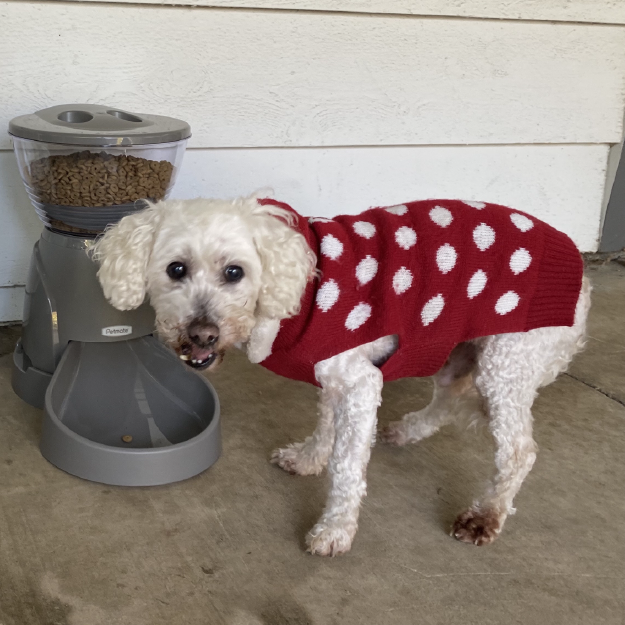
\includegraphics[width=1.5cm,height=1.5cm]{tikz/chapter10 - Diffusion Models Idea Image 1.png}};

\node[inner sep=0, outer sep=0, below=1.3cm of xt, xshift=4.05cm] (image2) at (0,0) {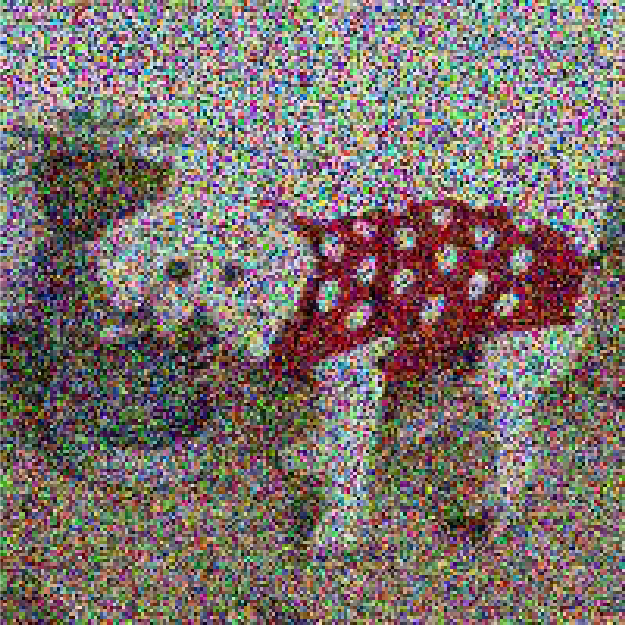
\includegraphics[width=1.5cm,height=1.5cm]{tikz/chapter10 - Diffusion Models Idea Image 2.png}};

\node[inner sep=0, outer sep=0, below=1.3cm of xT, xshift=8.1cm] (image3) at (0,0) {
\includegraphics[width=1.5cm,height=1.5cm]{tikz/chapter10 - Diffusion Models Idea Image 3.png}};

\draw[<-, bend left=45] ($(image.east)+(0.1cm,0.1cm)$) to node[above] {} ($(image2.west)+(-0.1cm,0.1cm)$);
\draw[->, bend right=45] ($(image.east)+(0.1cm,-0.1cm)$) to node[above] {} ($(image2.west)+(-0.1cm,-0.1cm)$);

\draw[<-, bend left=45] ($(image2.east)+(0.1cm,0.1cm)$) to node[above] {} ($(image3.west)+(-0.1cm, 0.1cm)$);
\draw[->, bend right=45] ($(image2.east)+(0.1cm,-0.1cm)$) to node[above] {} ($(image3.west)+(-0.1cm,-0.1cm)$);

\end{tikzpicture}
\end{document}